\documentclass[a4paper,11pt]{article}

%%%%%%%%%%%%%%%%%%%%%%%%%%%%%%%%%%%%%%%%%%%%%%%%%%%%%%%%%%%%%%%%%%%%%%%%
% Paquetes utilizados
%%%%%%%%%%%%%%%%%%%%%%%%%%%%%%%%%%%%%%%%%%%%%%%%%%%%%%%%%%%%%%%%%%%%%%%%

% Gráficos complejos
\usepackage{graphicx}
\usepackage{caption}
\usepackage{subcaption}
\usepackage{placeins}

% Soporte para el lenguaje español
\usepackage{textcomp}
\usepackage[utf8]{inputenc}
\usepackage[T1]{fontenc}
\DeclareUnicodeCharacter{B0}{\textdegree}
\usepackage[spanish]{babel}

% Código fuente embebido
\usepackage{listings}

% PDFs embebidos para el apéndice
\usepackage{pdfpages}

% Matemáticos
\usepackage{amssymb,amsmath}

% Tablas complejas
\usepackage{multirow}

% Formato de párrafo
\setlength{\parskip}{1ex plus 0.5ex minus 0.2ex}

%%%%%%%%%%%%%%%%%%%%%%%%%%%%%%%%%%%%%%%%%%%%%%%%%%%%%%%%%%%%%%%%%%%%%%%%
% Título
%%%%%%%%%%%%%%%%%%%%%%%%%%%%%%%%%%%%%%%%%%%%%%%%%%%%%%%%%%%%%%%%%%%%%%%%

% Título principal del documento.
\title{\textbf{Trabajo Práctico 1: Conjunto de Instrucciones MIPS}}

% Información sobre los autores.
\author{
  Andrés Gastón Arana, \textit{P. 86.203}                          \\
  \texttt{and2arana@gmail.com}                                     \\
  Sergio Matías Piano, \textit{P. 85.191}                          \\
  \texttt{smpiano@gmail.com}                                       \\ [2.5ex]
  \normalsize{2do. Cuatrimestre de 2012}                           \\
  \normalsize{66.20 Organización de Computadoras}                  \\
  \normalsize{Facultad de Ingeniería, Universidad de Buenos Aires}
}
\date{}

%%%%%%%%%%%%%%%%%%%%%%%%%%%%%%%%%%%%%%%%%%%%%%%%%%%%%%%%%%%%%%%%%%%%%%%%
% Documento
%%%%%%%%%%%%%%%%%%%%%%%%%%%%%%%%%%%%%%%%%%%%%%%%%%%%%%%%%%%%%%%%%%%%%%%%

\begin{document}

% ----------------------------------------------------------------------
% Top matter
% ----------------------------------------------------------------------
\thispagestyle{empty}
\maketitle

\begin{abstract}

  Este informe sumariza el desarrollo del trabajo práctico 1 de la materia
  Organización de Computadoras (66.20) dictada en el segundo cuatrimestre de
  2012 en la Facultad de Ingeniería de la Universidad de Buenos Aires.
  El mismo consiste en la construcción de un sistema halista de ordenamiento de
  archivos y el análisis de performance y perfilado del mismo, con foco en la
  utilización del conjunto de instrucciones de MIPS para soportar el
  desarrollo de estas tareas que será reutilizado en futuros trabajos
  prácticos.

\end{abstract}

\clearpage

% ----------------------------------------------------------------------
% Tabla de contenidos
% ----------------------------------------------------------------------
\tableofcontents
\clearpage


% ----------------------------------------------------------------------
% Desarrollo
% ----------------------------------------------------------------------
\part{Desarrollo}

\section{Introducción}

La utilización del conjunto de instrucciones MIPS nos permite generar código
assembly de los sistema de ordenamiento que anteriormente manejamos.
En este caso se realizara nuevamente el ordenamiento a través del algoritmo 
de stooge implementado a través del lenguaje ensamblador.

Ésto nos permite analizar nuevamente mediciones de tiempos de
ejecución y perfilado de performance a través de las herramientas \textit{time}
\cite{WIKITIME} y \textit{gprof} \cite{GPROF} para detectar y medir diferencias
de performance entre ambos algoritmos.

\section{Implementación}

El software que resuelve el problema planteado en el enunciado (disponible en
el anexo \ref{sec:enunciado}) fue implementado íntegramente en C y en especial
se agrega la implementación en assembly del algoritmo de stooge. El código
fuente de la solución está disponible en el anexo \ref{sec:source}.

El archivo stooge.S contiene la implementación del algoritmo de stooge en assembly
y la extensión \textit{S} refiere a que necesitamos que se lean las directivas
de precompilador.
Las directivas utilizadas nos permiten hacer referencia a los registros mediante
el nombre de los mismos.

En las siguientes secciones detallaremos las decisiones de diseño que
consideramos relevantes al desarrollo del trabajo práctico para algunos de
estos módulos.

\section{Compilación}

Se instrumentó un \textit{makefile} \cite{WIKIMAKE} para ejecutar las
instrucciones adecuadas de compilación para los distintos escenarios
requeridos.

\subsection{Ejecutable}

En el caso de la compilación del ejecutable final del trabajo práctico, la
tarea \textit{make} compila individualmente cada uno de los archivos fuente de
extensión \textit{c} y \textit{S} a través del ejecutable \textit{gcc} \cite{WIKIGCC}.
Los comandos utilizados para compilar cada uno de estos archivos fuente son los
siguientes:

\begin{lstlisting}
gcc -c -o build/obj/buffer.o source/buffer.c -I./source -Wall
gcc -c -o build/data.o source/data.c -I./source -Wall
gcc -c -o build/obj/clargs.o source/clargs.c -I./source -Wall
gcc -c -o build/obj/cltext.o source/cltext.c -I./source -Wall
gcc -c -o build/obj/tp1.o source/tp1.c -I./source -Wall
gcc -c -o build/obj/stoogec.o source/stooge.c -I./source -Wall
gcc -c -o build/obj/stoogeasm.o source/stooge.S -I./source -Wall
\end{lstlisting}

De este listado, cada una de las invocaciones obedece a la siguiente estructura
de argumentos:

\begin{description}

  \item[-c] Compila o ensambla el código fuente pero no corre el linker.  Por
    lo tanto la salida corresponde a un archivo objeto por cada archivo fuente.

  \item[-o] Especifica cual será el archivo de salida sea éste un archivo
    objeto, ejecutable, ensamblado o código preprocesado de C.

  \item[-Wall] Activa todos los mensajes de warning.

  \item[-I] Agrega el directorio especificado a la lista de directorios
    buscados para los archivos header

\end{description}

El resultado de la ejecución de estos comandos es que se generan archivos
objeto para cada fuente, listos para ser linkeados, en el directorio
\textit{build/obj}. Para realizar este último paso, se invoca nuevamente a
\textit{gcc} con un último comando:

\begin{lstlisting}
gcc -o build/tp0 \
  build/obj/buffer.o build/obj/data.o \
  build/obj/clargs.o build/obj/cltext.o \
  build/obj/tp1.o build/obj/stoogec.o build/obj/stoogeasm.o
\end{lstlisting}

El comando linkea todos los archivos objeto en un ejecutable final,
\textit{build/tp1}.

\subsection{Código de ensamblador MIPS}

En uno de los puntos del trabajo práctico, se pide visualizar el código en
ensamblador generado por el compilador en una arquitectura MIPS para el trabajo
práctico. Para completar esta tarea, se utiliza un comando utilizando
nuevamente \textit{gcc} que compila cada uno de los fuentes del trabajo
práctico, pero detiene el pipeline de compilación al generar el código de
ensamblador de cada uno de ellos. Los comandos correspondientes son los
siguientes:

\begin{lstlisting}
gcc -S -o build/obj/buffer.s source/buffer.c
gcc -S -o build/obj/data.s source/data.c
gcc -S -o build/obj/clargs.s source/clargs.c
gcc -S -o build/obj/cltext.s source/cltext.c
gcc -S -o build/obj/tp0.s source/tp0.c
gcc -S -o build/obj/stooge.s source/stooge.c
gcc -S -o build/obj/quicksort.s source/quicksort.c
\end{lstlisting}

En particular, el flag de compilación \textit{-S} es el que indica al
compilador que debe detener el pipeline al generar el código ensamblador para
el fuente compilado, de manera de que en el archivo indicado por \textit{-o} se
obtiene el código ensamblador pedido.

A modo informativo, existen indicativas opcionales como \textit{-mrnames}, que
nos permite indicarle al compilador que nombre los registros utilizados en el
código ensamblador en vez de numerarlos, y las indicativas \textit{-Ol}, con l
entre 0 y 3, que indican al compilador el nivel de optimización a desarrollar.

\section{Corridas de prueba}

Las corridas de prueba están automatizadas por el comando \(make\) \(testdata\) 
en la raíz del proyecto. Éstas corridas trabajan sobre el directorio de test.
Los comentarios se agregan en su ejecución.


\section{Análisis de tiempos de ejecución}

En las siguientes secciones detallaremos el proceso de análisis de tiempo de
ejecución realizado para los diferentes casos contemplados.

\subsection{Análisis previo}\label{sec:tiempos}

Para realizar el análisis de tiempos de ejecución se decidió elaborar un
conjunto de archivos de entrada para los cuales el tiempo de ejecución sería
medido. Se determinaron los siguientes criterios para generar los diferentes
experimentos a medir:

\begin{description}

  \item[Tamaño] Tanto los algoritmos de ordenamiento como el módulo
    de adquisición de entrada son sensibles al tamaño del archivo a ordenar. Se
    espera por lo tanto que a mayor tamaño aumenten los tiempos de ejecución.

  \item[Cantidad de lineas] Nuevamente, los algoritmos de ordenamiento son
    altamente sensibles a la cantidad de elementos a ordenar. Se espera que a
    mayor cantidad de lineas mayor sea el tiempo de ejecución del experimento.

  \item[Ordenamiento] Existe una dependencia entre el tiempo de ejecución de
    los algoritmos con el modo de ordenamiento de la entrada, es decir, si la
    entrada esta ordenada, inversamente ordenada o mezclada aleatoriamente. De
    acuerdo a la elección de la implementación del algoritmo \textit{quicksort}
    detallada en la sección \ref{sec:ord}, no se esperan grandes variaciones en
    los tiempos de ejecución para este algoritmo en este aspecto. Sin embargo
    \textit{stoogesort} es algo más lento en el caso de una entrada
    inversamente ordenada, por lo que se espera una diferencia apreciable de
    velocidad de ejecución para este caso.

\end{description}

\subsection{Generación de datos de entrada}

Se generaron archivos de texto base de 1\(Kb\), 8\(Kb\), 16\(Kb\) y
32\(Kb\). Para cada uno de esos archivos de texto se generaron 3 variantes
ordenadas según diferentes criterios:

\begin{enumerate}
  \item Ordenado con el comando `sort`.
  \item Ordenado inversamente con el comando `sort -r`.
  \item Mezclado aleatoriamente con el comando `sort -R`.
\end{enumerate}

Por último, se duplicaron todos los archivos generados introduciendo para cada
archivo una variante de lineas cortas. Estos archivos son idénticos en
contenido a los archivos originales, sólo que se procesaron un el comando
\textit{sed} \cite{WIKISED} para dividir las lineas largas del archivo original
en lineas de menos de 80 caracteres. De esta forma, se altera la cantidad de
lineas disponibles sin alterar el tamaño total del archivo.

De esta manera, se generaron en total 24 archivos distintos, cada uno
constituyendo un experimento diferente para cada uno de los parámetros
detallados en la sección \ref{sec:tiempos}.

\subsection{Mediciones}

Las mediciones realizadas en el trabajo practico 0 nos permitieron
encontrarnos con una diferencia importante respecto de la nueva 
implementación del algoritmo de ordenamiento stooge a través del uso
de las instruccinoes de MIPS 32.

Las medidas anteriormente tomadas son las siguientes:

\begin{enumerate}
  tiempo de ejecución de stoogesort original: 9.960s
  tiempo de ejecución de quicksort original: 0.143s
\end{enumerate}

Mientras que con la implementación en assembly obtenemos

\begin{enumerate}
  tiempo de ejecución de stoogesort mejorado: 4.230s
\end{enumerate}


\section{Diagramas de stack de cada función implementada en MIPS 32}

\subsection{String Compare Function}

La función string compare se declara de la siguiente manera

\begin{lstlisting}
  int compare_s(char* start, char* end);
\end{lstlisting}

Dicha función es una función hoja lo que nos está diciendo
que no llama a otra funciòn dentro de la declaraciòn de su cuerpo.
Tampoco utiliza espacio en memoria para alojar variables locales o bien
saved registers.
Como consecuencia estas funciones no necesitan alterar el registro sp.
Si es importante tener en cuenta que se tiene que alterar los registros
de argumentos para el pasaje de sus valores.

\subsection{Swap Function}

La funcion Swap se declara de la siguiente manera

\begin{lstlisting}
  void swap_s(char** data, unsigned int a, unsigned int b);
\end{lstlisting}

Y al ser una función hoja sucede lo mismo que con la anterior.
No contienen un stack propio.

\subsection{Stooge Sort Function}

La funcion Stooge Sort se declara de la siguiente manera

\begin{lstlisting}
  void stooge_sort(char** data, unsigned int a, unsigned int b);
\end{lstlisting}

En este caso la funcion llama a distintas funciones dentro
del desarrollo de su cuerpo.
Estas funciones son las anteriormente mencionadas como asì 
también se produce la llamada recursiva a sí misma.

El diagrama de stack que presenta se repite en caso que invoque
nuevamente la funcion pero alterando los registros de argumento
para que sus valores sean los correctos.

\begin{figure}
  \begin{subfigure}[b]{\textwidth}
    \centering
    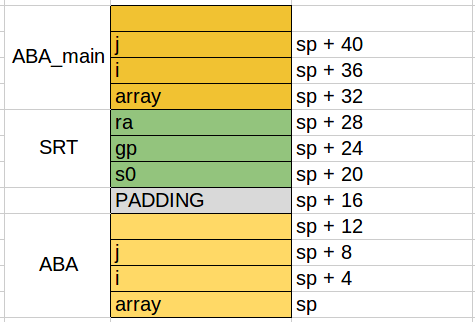
\includegraphics[width=\textwidth]{build/doc/stoogesort_diagrama.png}
    \caption{Stooge sort diagrama de stack}
  \end{subfigure}%
  \caption{Diagrama de Stack para la función de Stoogesort}\label{fig:speedup}
\end{figure}

\FloatBarrier

\section{Conclusiones}

Respecto de las mediciones que obtuvimos luego de desempeñarnos con el
conjunto de instrucciones que MIPS nos brinda nos hemos sorprendido 
justmente en los tiempos de procesamiento.
Hemos visto un claro progreso y mejora con el algoritmo de 
ordenamiento implementado en assembly que nos permitiò mejorar el 
marcado por el mismo algoritmo pero desarrollado en c.

Nos resulto complicado de desarrollar a la hora de querer realizar verificaciones
y comprobar que los datos que iban pasando eran los que esperabamos.
Un mininmo error que se produzca y puede ser que el codigo no haga lo que
queremos hacer.

Por otro lado, coincidimos que gracias al poder manejarnos con las instrucciones
de MIPS mejoramos mucho el tiempo que se demora en ir a leer los datos a memoria
o bien almacenarlos en ella.
\cite{OPT}.

\begin{thebibliography}{99}

\bibitem{WIKISORT} Sort, file sorting linux command, http://en.wikipedia.org/wiki/Sort\_(Unix)
\bibitem{WIKIQS} Quicksort, fast sorting algorithm, http://en.wikipedia.org/wiki/Quicksort
\bibitem{WIKIST} Stoogesort, inefficient sorting algorithm, http://en.wikipedia.org/wiki/Stooge\_sort
\bibitem{WIKITIME} Time, execution time measurement linux command, http://en.wikipedia.org/wiki/Time\_(Unix)
\bibitem{GPROF} GNU gprof, profiling utility for compiled executables, http://www.cs.utah.edu/dept/old/texinfo/as/gprof.html
\bibitem{WIKIBUB} Bubblesort, simple sorting algorithm, http://en.wikipedia.org/wiki/Bubblesort
\bibitem{WIKISED} Sed, stream editor linux command, http://en.wikipedia.org/wiki/Sed
\bibitem{WIKIBASH} Bash, bourne again linux shell, http://en.wikipedia.org/wiki/Bash\_(Unix\_shell)
\bibitem{WIKIRUBY} Ruby, dynamic, reflective general purpose language, http://en.wikipedia.org/wiki/Ruby\_(programming\_language)
\bibitem{OPT} Knuth, Donald (December 1974). "Structured Programming with go to Statements". ACM Journal Computing Surveys 6 (4): 268.
\bibitem{WIKIMAKE} Make, automatic source code building utility, http://en.wikipedia.org/wiki/Makefile
\bibitem{WIKIGCC} GCC, GNU Compiler Collection, http://en.wikipedia.org/wiki/GNU\_Compiler\_Collection

\end{thebibliography}

\clearpage

\part{Apéndice}
\appendix

\section{Enunciado original}\label{sec:enunciado}
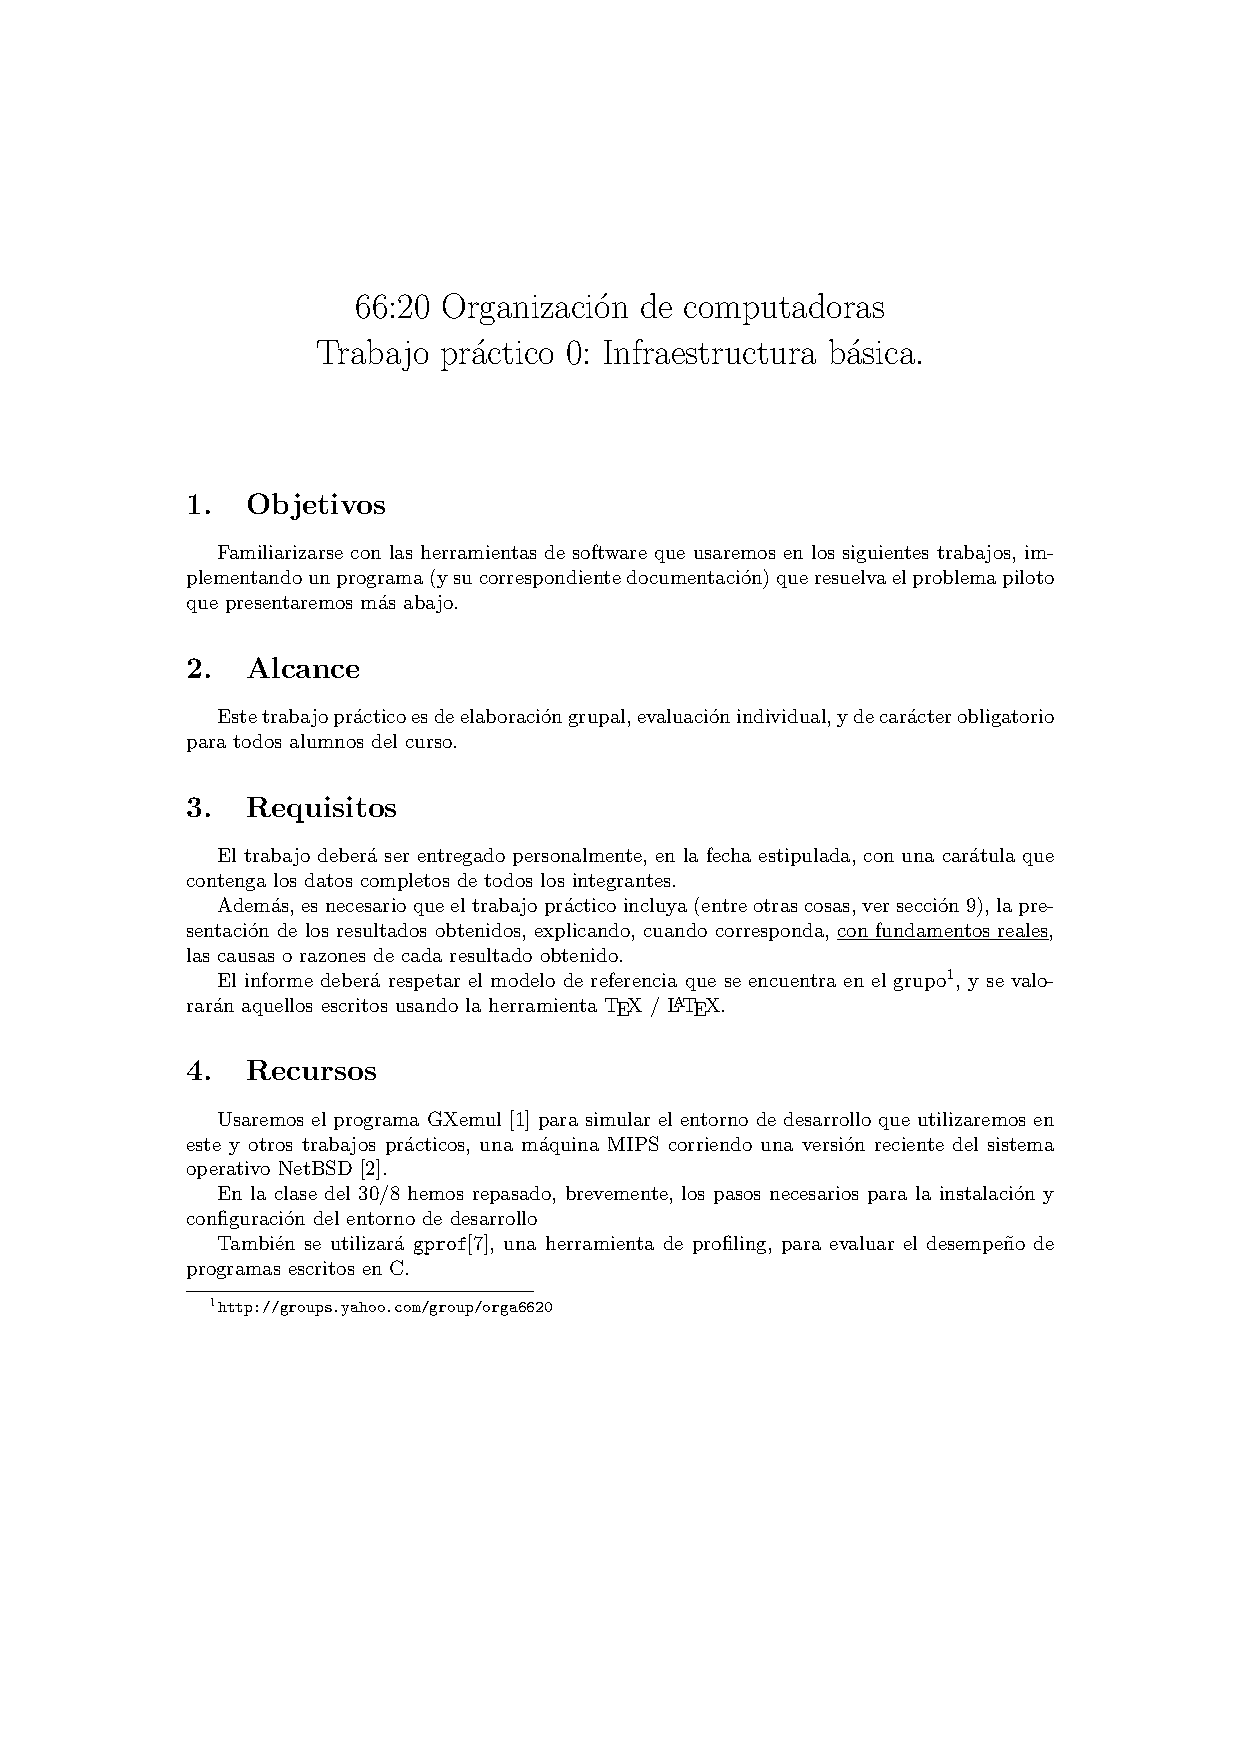
\includepdf[pages={-}]{docs/enunciado.pdf}

\clearpage
\section{README del material digital}\label{sec:readme}
\includepdf[pages={-}]{build/doc/README.pdf}

\clearpage
\section{Salida de gprof}\label{sec:gprof}
\clearpage
\lstset{
  basicstyle=\footnotesize,
  showspaces=false,
  showstringspaces=false,
  breaklines=true,
  frame=single
}

\lstinputlisting{prof/results}

\clearpage
\section{Código fuente}\label{sec:source}
\clearpage
\definecolor{gray}{rgb}{0.5,0.5,0.5}
\lstset{
  language=C,
  title=\lstname,
  basicstyle=\footnotesize,
  showspaces=false,
  showstringspaces=false,
  breaklines=true,
  commentstyle=\color{gray},
  numbers=left,
  numberstyle=\tiny\color{gray},
  numbersep=5pt,
  frame=single
}



 NOTA: Sólo se incluyen los fuentes de los archivos que fueron agregados y alterados.

\lstinputlisting{source/stooge.h}
\lstinputlisting{source/stooge.c}
\lstinputlisting{source/stooge.S}
\lstinputlisting{source/tp1.c}

\end{document}
